\chapter{Método espectral e Método dos elementos finitos}
\label{cap:I}
\section{sobre}\corr{Sério? O título é sobre?}

 Método espectral é um método poderoso usado para solução de equações diferencial parcial. Diferentemente do método das diferenças finitas, que considera apenas os pontos próximos do ponto que queremos computar chamada de método \emph{local}, o método espectral considera todo o domínio, sendo assim um método \emph{global}. Essa técnica tem mais precisão pois converge exponencialmente diferente do método local. É preferível a utilização desse método quando a solução varia em função do \textit{tempo} e \textit{espaço}. \corr{E o método de elementos espectrais?}

\section{Interpolação}
 A interpolação de uma função $f(x)$ por um polinômio trigonométrico ou não, de grau $n$, $P_{n}(x)$ e que satisfaça:

\begin{equation}
	P_n (x_i) = f(x_i) \ i = 1,2,...,\emph{n+1}
\end{equation}

 Onde $f(x_i)$ é a função $f$ pré-calculada nos pontos $x_i$. A escolha desses pontos $x_i$ ainda será explicada.

\subsection{Interpolação polinomial}
 \begin{figure}[!ht]
  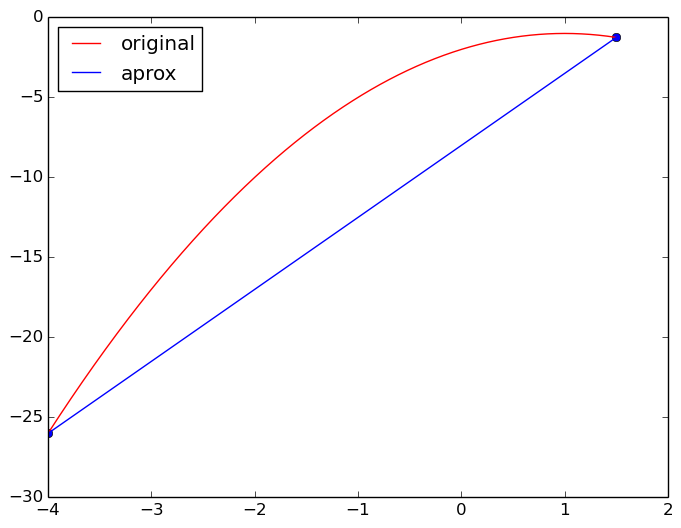
\includegraphics[width=0.7\textwidth,center]{figuras/interpolacao_linear.png}
  \caption{interpolação simples}
\end{figure}

 Antes do uso de calculadoras e computadores, um método de estimar o valor de uma $f$ num ponto, era utilizar tabelas com valores de pré-calculados. \corr{A maneira mais simples de entender é a estimação do valor da função em um ponto intermediário entre dois pontos conhecidos é o uso da interpolação \emph{Linear}}.

\begin{equation}
	f(x) \approx \frac{x - x_1}{x_0 - x_1}f(x_0)  + 							 \frac{x - x_0}{x_1 - x_0}f(x_1)
\end{equation} 
 
 Para fazermos essa interpolação para $n$ pontos conhecidos aproximamos uma função usando o polinômio base de \emph{Lagrange}.
\begin{equation}
C_i(x) = \prod_{j = 0 \\ j \neq i}^{N} \frac{x - x_j}{x_i - x_j} 
\end{equation}

\begin{figure}[!h]
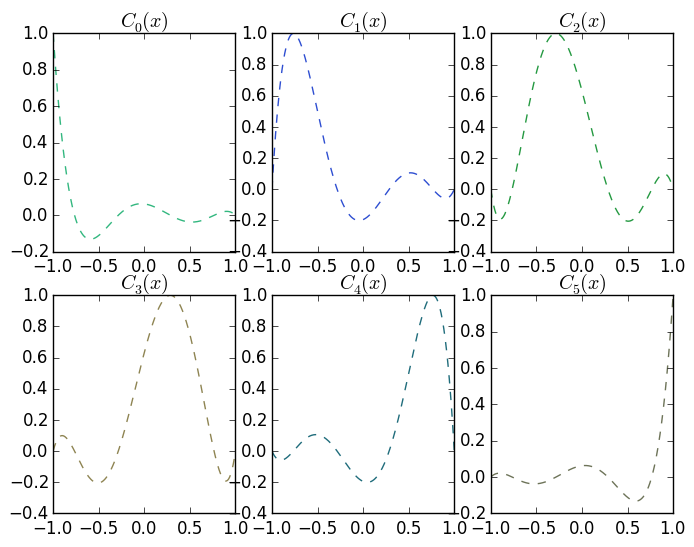
\includegraphics[width=0.7\textwidth, center ]{figuras/exemplo_polinomio_lagrange.png}
\caption{polinômio base de Lagrange para 6 pontos}
\end{figure}

 A interpolação de \emph{Lagrange} é dada por :
\begin{equation}
 P_n(x) \equiv \sum_{i = 0}^{N} f(x_i)C_i(x) 
\end{equation}
 Obedecendo que $P_n(x_i) = f(x_i)$. Apesar dos pontos interpoladores equidistante serem comumente utilizados, não há restrições, podendo até mesmo estar fora de ordem.
\begin{figure}[h]
  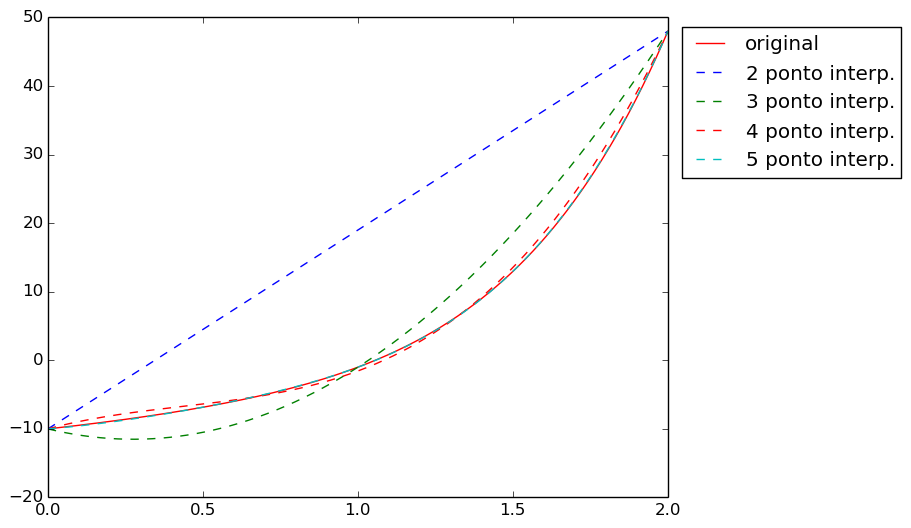
\includegraphics[width=0.5\textwidth, center]{figuras/interpolacao_linear5.png}
  \caption{interpolação com n pontos equidistantes}
\end{figure}

\pagebreak
\newpage

\subsection{Fenômeno de Runge}
 Apesar de parecer que uma boa interpolação tenha uma boa aproximação usando pontos igualmente distantes sobre um interval $[a,b]$, $\lim_{n \rightarrow \infty} |f(x) - P_n(x)| = 0$ para qualquer $f(x)$ diferenciável.
 No início do século XX, \emph{Carl David Tolmé Runge}, provou que para uma função $f(x)$:
 \begin{equation}
 f(x) = \frac{1}{1 + x^2} , x \in [-5,5]
 \end{equation}
 que para pontos equidistantes, a interpolação converge apenas no intervalo $[-3.63,3.63]$, e diverge fora do mesmo. Para polinômios de maior grau, esse intervalo de convergência tende a diminuir e perto dos pontos de fronteira diverge bastante (figura abaixo).

\begin{figure}[htp]
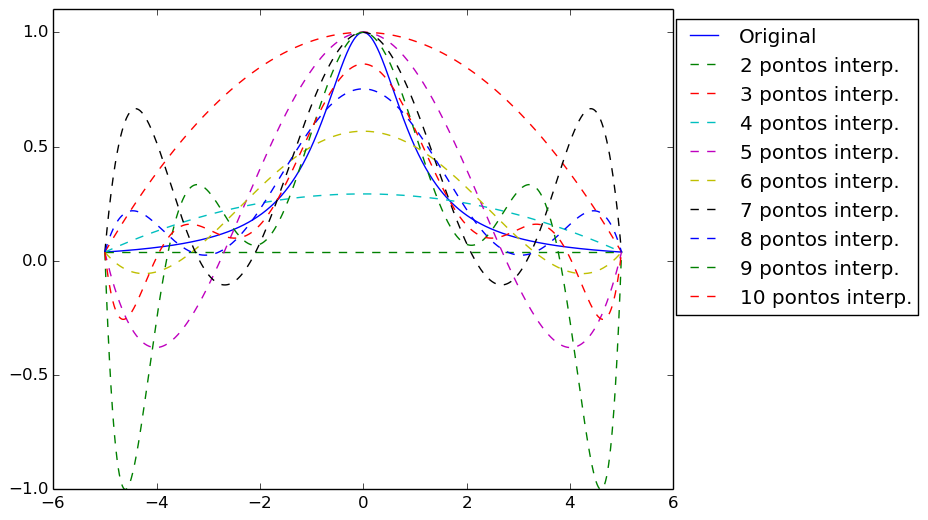
\includegraphics[width=0.7\textwidth, center]{figuras/fenomeno_runge.png}
\caption{fenômeno Runge}
\end{figure}

 Assim, Runge prova que no meio do intervalo temos boas aproximações mas infelizmente perto dos extremos, os valores interpolados oscilam muito, para um polinômio de grau n com pontos equidistante. Esse fenômeno sugere que escolhamos pontos diversos que tenham menor concentração do meio do intervalo, onde temos uma maior precisão, e aumentar a densidade de pontos próximos dos extremos.
 Agora como encontrar uma distribuição de pontos de forma que melhore a interpolação ? A resposta pode ser explicado pelos teoremas a seguir.
 
\subsection{ Teorema I: Erro de interpolação de Cauchy}

 Dado $f(x)$  com pelo menos $N+1$ derivadas no intervalo de interesse e seja $P_N(x)$ seja o interpolador Lagrangiano de grau $N$. Então o erro é dado por:
 
 \begin{equation}
 f(x) - P_N(x) = \frac{1}{[N+1]!}f^{(N+1)}(\epsilon)\prod^{N}_{i = 0} (x - x_i)
 \end{equation}
 Para um $\epsilon(x) \in [-1,1]$.
 
 Logo, para minimizar o erro, não podemos fazer nada quanto o termo $f^(N+1)(\epsilon)$, pois necessita conhecer a função interpolada. Quanto o polinômio $\prod^{N}_{i = 0} (x - x_i)$, sabemos que o coeficiente do termo $x^N$ é $1$, independente da escolha de pontos. Então a pergunta que fica é, qual escolha de pontos nos dá um \emph{polinômio} com coeficiente líder igual a $1$ minimiza essa função ? Felizmente e coincidentemente, essa resposta foi respondida quase meio século antes do próprio fenômeno de Runge ser descoberto. Veremos no próximo teorema.

 
\subsection{Teorema II: Amplitude minima}
 De todos os polinômios de grau $N$ com coeficiente de $x^N$ igual a 1, o único polinômio que tem o menor máximo no intervalo $[-1,1]$ é $\frac{T_N(x)}{2^{N-1}}$, o polinômio de \emph{Chebyshev} \corr{dividido por ideia}. Em outras palavras, todos os polinômios de mesmo grau e coeficiente líder unitário, satisfazem a desigualdade: \corr{Em Inglês o nome deste tipo de polinômio é ``monic polynomial''}

\begin{equation}
	max_{x \in [-1,1]}|P_N(x)| \geq  max_{x \in [-1,1]} \left |\frac{T_N(x)}{2^{N-1}}  \right |  = \frac{1}{2^{N-1}}\\
\end{equation}

\corr{Você erra sistemáticamente expoentes em \LaTeX : $x^{1+2}$ ou $x^{(1+2)}$ e não $x^(1+2)$}

\begin{align}
    T_0(x) &= 1\\
    T_1(x) &= x\\
    T_{N+1}(x) &= 2xT_N(x) - T_{N-1}(x)\\
    T_{N}(x)&=\cos(n \arccos x)=\cosh(n\,\operatorname{arcosh}\,x)
\end{align}\corr{Tem que colocar} \& \corr{onde você quer alinhar as equações!!!}

 Agora, qualquer polinômio de grau $N$, com coeficiente líder unitário, pode ser fatorado na forma de um produtório  $(x - x_i)$, onde $x_i$ é uma das raízes do polinômio, em particular: 
 \begin{equation}
 \frac{1}{2^N}T_{N+1}(x) \equiv \prod_{i = 1}^{N+1} (x-x_i)
 \end{equation}
 Temos então que, para minimizar o erro no \emph{Teorema I}, o polinômio deve ser proporcional a $T_{N+1}(x)$. Isso implica que  os pontos interpoladores que minimizam o erro, são as raízes do próprio polinômio de \emph{Chebyshev} de grau $N+1$.
 
 Usando o fato que esse polinômio pode ser reescrita como uma função trigonométrica, temos que as raízes são:
 \begin{equation}
  x_i  \equiv \cos \left [ \frac{(2i - 1)\pi}{2(N+1)}  \right ] , i = 1,2,..., N+1
 \end{equation}
 
 Pela expansão de \emph{Taylor} da função coseno, verificamos a afirmação de acima que o espaçamento da malha é $O(N^2)$ perto das fronteiras:
 
 \begin{equation}
  x_1 \approx -1 + \frac{\pi^2}{8N^2}\ ;\ x_2 \approx -1 + \frac{9\pi}{8N^2} [N\gg 1]
 \end{equation}
 
 Agora temos como conseguir o polinômio de \emph{Chebyshev} que minimiza o erro. Porém essa escolha de polinômio varia para diferentes geometrias ou funções harmônicas ou hermitianas.
 \begin{figure}[b]
 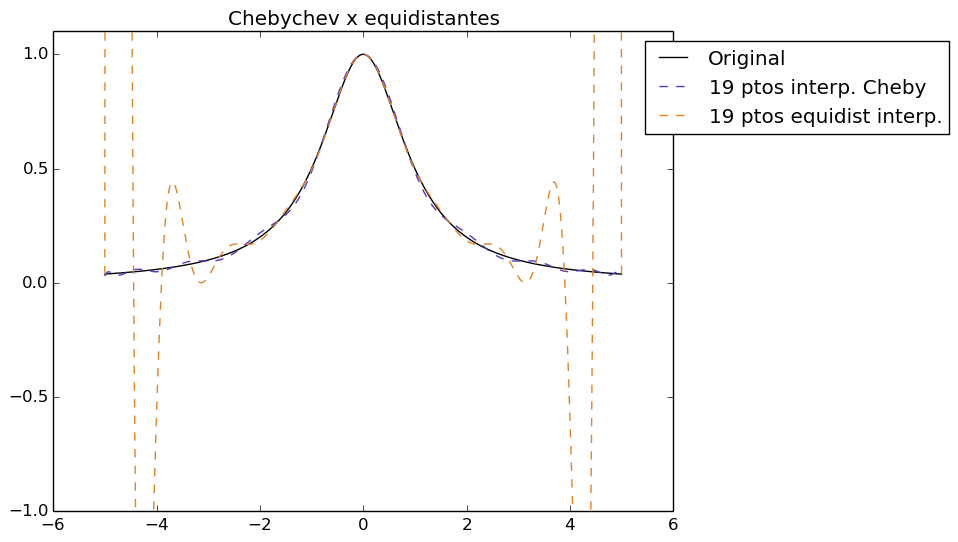
\includegraphics[width=0.45\textwidth, center]{figuras/chebychev_equidist.png}
 \caption{método de raízes de chebychev contra raízes de pontos equidistante}
 \end{figure}
\pagebreak
\subsection{Integração gaussiana e linhas pseudoespectral}
\corr{Eu colocaria em outra seção e não como subseção da interpolação}
 A razão pelo qual o método de colocação é também chamado "pseudoespectral" devido a colocação otimizada dos pontos de interpolação, como o polinômio de \emph{Chebyshev}, faz o método da colocação idêntico ao método de \emph{Galerkin} se o produto interno é calculado por um tipo de integração numérica conhecida como Integração gaussiana. \corr{Você não falou o que é o método espetral, Galerkin, etc}
 Integração numérica e interpolação Lagrangiana são muito correlacionada pois o método de integração é de aproximar o polinômio pelo integrando de $f(x)$ e depois integrar $P_N(X)$. Como o interpolado pode ser integrado facilmente, o erro é dado como a diferença de $f(x)$ e $P_N(x)$.  A fórmula é dada por:
 \begin{equation}
  \int_a^b f(x) \partial x \approx \sum_{i = 0}^N w_i f(x)
 \end{equation}
 e a função peso $w_i$ é dado por:
 \begin{equation}
  w_i \equiv \int_{a}^{b} C_i(x) \partial x
 \end{equation}
 Onde $C_i$ é o polinômio base de \emph{Lagrange}.
 Quando calculamos, os pontos de \emph{interpolação} são nomeados de \emph{abcissas}, enquanto que a \emph{integral} de um polinômio base é chamado de \emph{quadratura}, no contexto da integração numérica.
 
 A \emph{ordem} de um método numérico é diretamente relacionado a maior polinômio que o aproxima. Por exemplo quando aplicamos a interpolação para equações de primeiro e segundo grau, os erros são respectivamente $O(h^2),\ O(h^4)$. Similarmente, a fórmula de quadratura com $(N + 1)$ pontos, será exata se o integrado for um polinômio de grau $N$.
 
 Gauss fez uma observação que pontos de interpolação equidistantes não são tão bons. Se tivermos pontos interpoladores $x_i$ e seus pesos $w_i$ 
desconhecido, teremos o dobro de parâmetros para escolher que maximizem a precisão do método e assim podemos ter uma aproximação exata para polinômios de grau $(2N + 1)$.
\subsection{Teorema: Integração Gauss-Jacobi}
 Seja $(N + 1)$ pontos interpoladores $x_i$ escolhidos e raízes de $P_N(x)$, um polinômio de grau $(N+1)$ do tipo \emph{ortogonal} no intervalo $[a,b]$ com respeito a função $p(x)$, então a fórmula de quadratura é dado por:
\begin{equation}
 \int^a_b f(x)p(x) \partial x = \sum^{N}_{i= 0} w_i f_i(x)
\end{equation} 
é exata para toda $f(x)$ polinomial de grau máximo $(2N +1)$

\subsection{tipos de polinômio}
	adicionar outros polinômios de base talvez ?
	Gauss-Jacobi
	Gauss-Lobatto-Jacobi
	Gauss-Radau-Jacobi 


\subsection{Derivada}
	As derivadas podem ser calculadas da seguinte forma:
	\begin{align}
	f(x) = \sum^{N-1}_{i=0} f(x_i) C_i(x)\\
	\frac{\partial f(x)}{\partial x} = \sum^{N}_{i = 0} f(x_i) \frac{\partial C_i(x)}{\partial x}
	\end{align}
	para calcular as integrais, é necessário conhecer a derivada nos nós da quadratura, $x_i$ :
	%\begin{equation}
	%
	%\end{equation}

\section{método dos elementos finitos}
adicionar texto de elementos dinâmicos